\documentclass[12pt,a4paper]{article}

\input{/home/tabaka/Documents/GitHub/Defs/defs.tex}

\setcounter{zadaniaRozdzial}{1}
%\pagestyle{empty}

\begin{document}
	\begin{center}
		\LARGE Trygonometria
	\end{center}
	\vspace{1cm}
	
	\ZbiorZadanie{Wyznacz funkcje trygonometryczne kątów ostrych trójkąta egipskiego, czyli trójkąta o bokach długości $3$, $4$ i $5$.}
	
	\ZbiorZadanie{
		Wyznacz funkcje trygonometryczne podanych kątów:
		\begin{figure}[h]
			\centering
			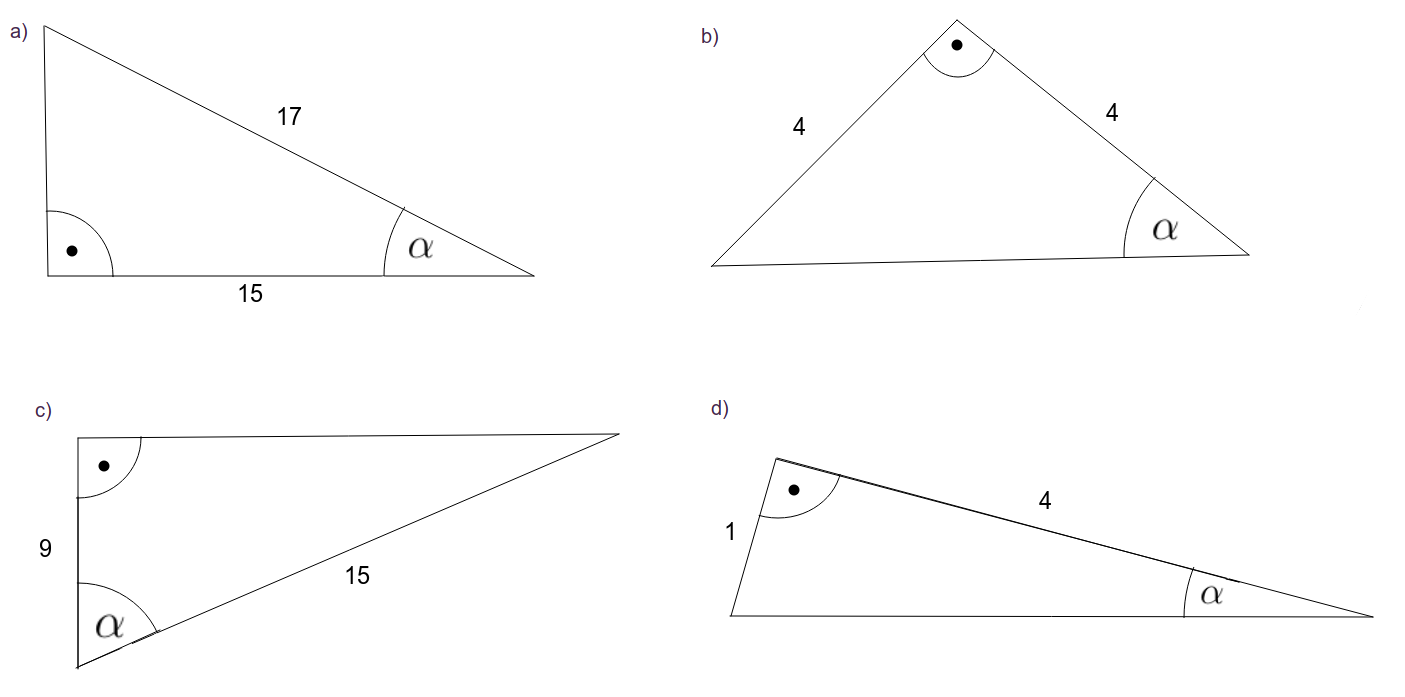
\includegraphics[scale=0.35]{t1}
		\end{figure}
	}
	
	\ZbiorZadanie{
		Oblicz długości brakujących boków:
		\begin{figure}[h]
			\centering
			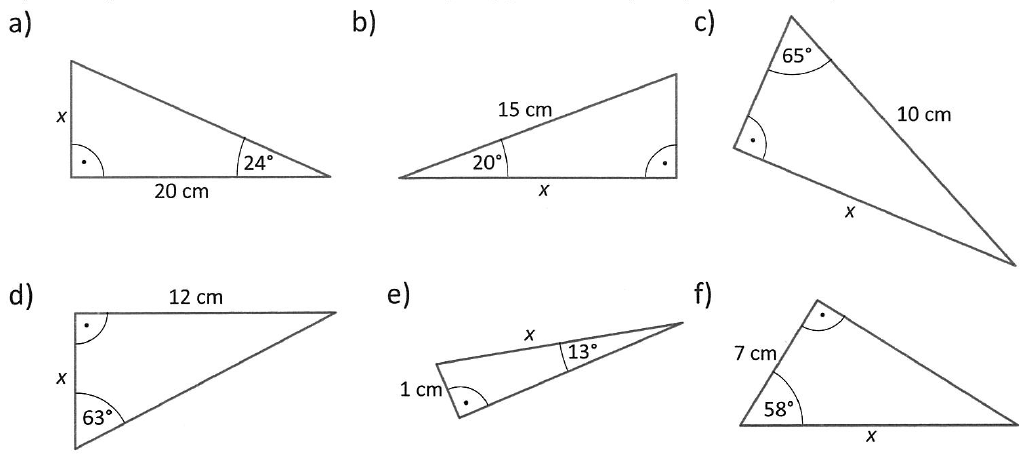
\includegraphics[scale=0.65]{t2}
		\end{figure}
	}
	
	\newpage
	
	\ZbiorZadanieTwoXThree{Dla podanej funkcji trygonometrycznej kąta ostrego $\alpha$ wyznacz wartości pozostałych funkcji trygonometrycznych:}
	{$\sin\alpha=\frac{5}{13}$}
	{$\cos\alpha=0{,}5$}
	{$\cos\alpha=\frac{\sqrt{5}}{5}$}
	{$\ctg\alpha=\frac{1}{\sqrt{3}}$}
	{$\tg\alpha=2$}
	{$\sin\alpha=\frac{1}{\sqrt{3}}$}
	
	\ZbiorZadanie{
		Oblicz:
		\begin{enumerate}[a)]
			\item $4\cdot\cos(60^\circ)\cdot\sin(30^\circ)-\cos(30^\circ)\cdot\sin(30^\circ)=$
			\item $\text{ctg }(30^\circ)\cdot\text{ctg }(45^\circ):(\text{ctg }(60^\circ)\cdot\text{tg }(45^\circ))=$
			\item $18\cdot\sin(30^\circ)\cdot\text{tg }(30^\circ):(\cos(30^\circ)\cdot\text{tg }(60^\circ))=$
			\item $6\cdot(\sin(30^\circ)\cdot\cos(45^\circ)\cdot\text{ctg }(60^\circ)):(\text{ctg }(30^\circ)\cdot\sin(45^\circ))=$
			\item $12\cdot(\text{tg }(60^\circ)-\cos(60^\circ))\cdot(\text{tg }(30^\circ)+\text{tg }(30^\circ)+\cos(30^\circ))=$
			\item $(\sin(45^\circ)+\text{ctg }(45^\circ))\cdot(6\cdot\sin(60^\circ)-\text{ctg }(30^\circ))=$
			\item $(\cos(45^\circ)-\cos(30^\circ))\cdot(\cos(45^\circ)+\cos(30^\circ))=$
			\item $(3\cdot\sin(45^\circ)+\text{tg }(60^\circ))\cdot(3\cdot\sin(45^\circ)-\text{tg }(60^\circ))=$
			\item $(\sin(60^\circ)+\cos(30^\circ))^2-(\sin(30^\circ)+\cos(60^\circ))^2=$
		\end{enumerate}
	}
	
	\ZbiorZadanieTwoXTwo{Sprawdź, czy podana równość jest tożsamością trygonometryczną:}
	{$\tg\alpha\cdot\cos\alpha=\sin\alpha$}
	{$\sin\alpha\left(\frac{1}{\sin\alpha}-\sin\alpha\right)=\cos^2\alpha$}
	{$1-2\sin^2\alpha=2\cos^2\alpha$}
	{$\sin\alpha+\sin\alpha\cdot\text{tg }^2\alpha=\frac{\text{tg }\alpha}{\cos\alpha}$}
	
	\ZbiorZadanie{Promienie słoneczne padają na drzewo pod kątem $25^\circ$. Wiedząc, że drzewo rzuca cień o długości $30\,\text{m}$, oblicz wysokość drzewa.}
	
	\ZbiorZadanie{Promienie słoneczne padają pod kątem $16^\circ$ na maszt o wysokości $15{,}5\,\text{m}$. Oblicz długość cienia rzucanego przez maszt.}
	
	\ZbiorZadanieTwoXThree{Do ramienia końcowego kąta $\alpha$ należy punkt $P$. Oblicz wartości funkcji trygonometrycznych tego kąta, jeśli:}
	{$P=(5,12)$}
	{$P=(-5,12)$}
	{$P=(-3,-4)$}
	{$P=(1,-2)$}
	{$P=(-\sqrt{3},\sqrt{6})$}
	{$P=(-\sqrt{5},-\sqrt{15})$}
	
	\ZbiorZadanieTwoXThree{Dla podanej funkcji trygonometrycznej kąta $\alpha$ wyznacz wartości pozostałych funkcji trygonometrycznych, jeśli $\alpha\in(90^\circ,180^\circ)$:}
	{$\sin\alpha=\frac{5}{13}$}
	{$\cos\alpha=-0{,}5$}
	{$\cos\alpha=-\frac{\sqrt{5}}{5}$}
	{$\ctg\alpha=-\frac{1}{\sqrt{3}}$}
	{$\tg\alpha=-2$}
	{$\sin\alpha=\frac{1}{\sqrt{3}}$}
	
	\ZbiorZadanieTwoXThree{Oblicz, korzystając ze wzorów redukcyjnych:}
	{$\sin 120^\circ=$}
	{$\cos 120^\circ=$}
	{$\sin 150^\circ=$}
	{$\tg 150^\circ=$}
	{$\sin 225^\circ=$}
	{$\cos 420^\circ=$}
	
	\ZbiorZadanieTwoXThree{Oblicz, korzystając ze wzorów redukcyjnych:}
	{$\cos 330^\circ=$}
	{$\sin(-210^\circ)=$}
	{$\tg 210^\circ=$}
	{$\sin 1050^\circ=$}
	{$\cos(-600^\circ)=$}
	{$\tg(-450^\circ)=$}
	
	\ZbiorZadanieTwoXThree{Dany jest trójkąt o bokach $a$ i $b$ oraz kącie $\gamma$ między tymi bokami. Oblicz pole tego trójkąta, jeśli:}
	{$a=3,\; b=4,\; \gamma=30^\circ$}
	{$a=8,\; b=4\sqrt{2},\; \gamma=45^\circ$}
	{$a=7,\; b=\sqrt{3},\; \gamma=60^\circ$}
	{$a=4\sqrt{2},\; b=5\sqrt{6},\; \gamma=120^\circ$}
	{$a=\frac{13\sqrt{2}}{11},\; b=11,\; \gamma=135^\circ$}
	{$a=1,\; b=1,\; \gamma=150^\circ$}
	
	\ZbiorZadanie{Oblicz pole trójkąta równoramiennego o ramionach długości $6\,\text{cm}$ i kącie między nimi równym $120^\circ$.}
	
	\ZbiorZadanie{Pole rombu jest równe $108\,\text{cm}^2$, a jedna z jego przekątnych ma długość $18\,\text{cm}$. Oblicz długość drugiej przekątnej.}
	
	\ZbiorZadanieTwoXThree{Dany jest równoległobok o bokach $a$ i $b$ oraz kącie $\gamma$ między tymi bokami. Oblicz pole tego równoległoboku, jeśli:}
	{$a=8,\; b=6,\; \gamma=30^\circ$}
	{$a=14,\; b=\frac{\sqrt{2}}{7},\; \gamma=45^\circ$}
	{$a=4,\; b=\sqrt{3},\; \gamma=60^\circ$}
	{$a=3\sqrt{6},\; b=3\sqrt{2},\; \gamma=120^\circ$}
	{$a=5\sqrt{2},\; b=11,\; \gamma=135^\circ$}
	{$a=\frac{1}{2},\; b=\frac{1}{3},\; \gamma=150^\circ$}
	
	\ZbiorZadanie{Dany jest równoległobok o bokach długości $10\,\text{cm}$ i $12\,\text{cm}$ oraz kącie rozwartym równym $150^\circ$. Oblicz różnicę długości wysokości tego równoległoboku.}
	
	\ZbiorZadanie{Oblicz sinus kąta ostrego rombu o przekątnych długości $12\,\text{cm}$ i $16\,\text{cm}$.}
	
	\newpage
	
	\begin{center}
		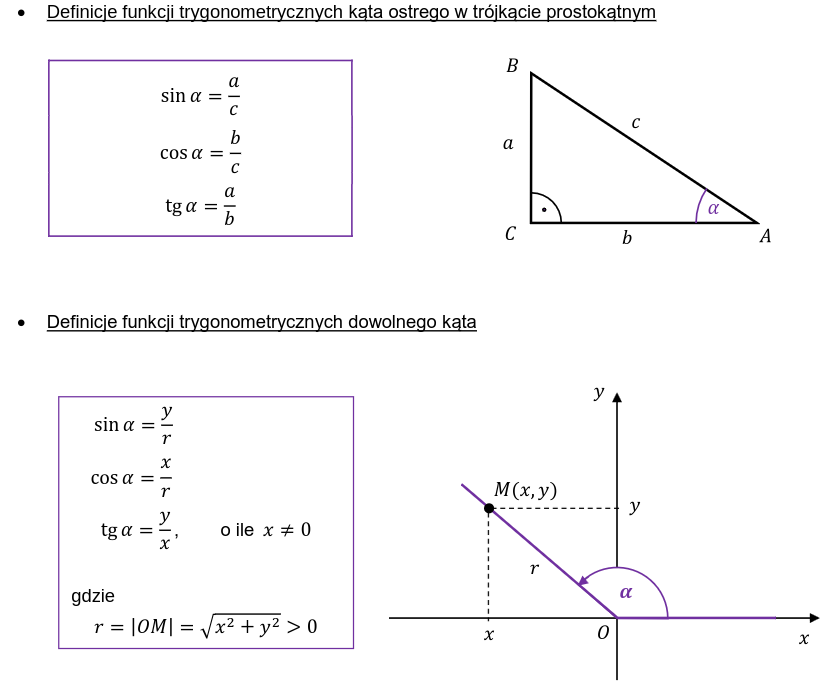
\includegraphics[width=15cm]{wzory}
	\end{center}
	
	\begin{center}
		\renewcommand{\arraystretch}{1.5}
		\begin{tabular}{|c|c|c|c|c|c|}
			\hline
			& $0^\circ$ & $30^\circ$ & $45^\circ$ & $60^\circ$ & $90^\circ$ \\
			\hline
			$\sin\alpha$
			& $0$
			& $\frac{1}{2}$
			& $\frac{\sqrt{2}}{2}$
			& $\frac{\sqrt{3}}{2}$
			& $1$ \\
			\hline
			$\cos\alpha$
			& $1$
			& $\frac{\sqrt{3}}{2}$
			& $\frac{\sqrt{2}}{2}$
			& $\frac{1}{2}$
			& $0$ \\
			\hline
			$\tg\alpha$
			& $0$
			& $\frac{\sqrt{3}}{3}$
			& $1$
			& $\sqrt{3}$
			& \text{nie istnieje} \\
			\hline
		\end{tabular}
	\end{center}
	
	\WzorElastyczny{
		\begin{center}
			\begin{tabular}{p{5cm} p{5cm} p{5cm}}
				$\sin(90^\circ-\alpha)=\cos\alpha$
				&
				$\cos(90^\circ-\alpha)=\sin\alpha$
				&
				\\[6pt]
				$\sin(90^\circ+\alpha)=\cos\alpha$
				&
				$\cos(90^\circ+\alpha)=-\sin\alpha$
				&
				\\[6pt]
				$\sin(180^\circ-\alpha)=\sin\alpha$
				&
				$\cos(180^\circ-\alpha)=-\cos\alpha$
				&
				$\tg(180^\circ-\alpha)=-\tg\alpha$
				\\[6pt]
				$\sin(180^\circ+\alpha)=-\sin\alpha$
				&
				$\cos(180^\circ+\alpha)=-\cos\alpha$
				&
				$\tg(180^\circ+\alpha)=\tg\alpha$
			\end{tabular}
		\end{center}
	}
	
	\WzorElastyczny{
		\begin{center}
			\begin{tabular}{p{5cm} p{5cm} p{5cm}}
				$\sin(k\cdot360^\circ+\alpha)=\sin\alpha$
				&
				$\cos(k\cdot360^\circ+\alpha)=\cos\alpha$
				&
				$\tg(k\cdot180^\circ+\alpha)=\tg\alpha$
				\\[6pt]
				$\sin(-\alpha)=-\sin\alpha$
				&
				$\cos(-\alpha)=\cos\alpha$
				&
				$\tg(-\alpha)=-\tg\alpha$
			\end{tabular}
		\end{center}
	}
	
\end{document}